% Model report generated by SolverMapp.
% Compile with: pdflatex, bibtex, pdflatex, pdflatex (references.bib is written by the first run).
\begin{filecontents*}[overwrite]{references.bib}
@misc{chenciner2000,
  author = {Chenciner \& Montgomery},
  year   = {2000},
  note   = {Chenciner, A., Montgomery, R. (2000). A remarkable periodic solution of the three-body problem in the case of equal masses. Annals of Mathematics, 152, 881-901.}
}

@misc{ref,
  note   = {Total mechanical energy (kinetic + gravitational potential), conserved},
  key    = {Total mechanical energy (kinetic + gravi}
}
\end{filecontents*}
\documentclass[11pt,a4paper]{article}
\usepackage[T1]{fontenc}
\usepackage[utf8]{inputenc}
\usepackage{lmodern}
\usepackage{amsmath,amssymb}
\usepackage{booktabs,longtable}
\usepackage{siunitx}
\usepackage{algorithm}
\usepackage{algpseudocode}
\usepackage{tikz}
\usetikzlibrary{positioning,shapes.geometric,shapes.misc,arrows.meta}
\usepackage{adjustbox}
\usepackage[hidelinks]{hyperref}

\title{Three-body problem: figure-eight orbit}
\author{}
\date{\today}

\begin{document}
\maketitle

The model consists of 7 equations in 12 variables: 5 inputs, 6 state variables, 0 intermediate variables and 1 output. It is solved in 2 steps (Algorithm~\ref{alg:solution}).

\section{Nomenclature}
\begin{longtable}{@{}l p{0.48\linewidth} l l@{}}
  \toprule
  Symbol & Description & Unit & Value \\
  \midrule
  \endhead
  \bottomrule
  \endfoot
  \multicolumn{4}{@{}l}{\textit{Inputs}} \\
  $t$ & Time & \si{s} & \num{0} \\
  $G$ & Gravitational constant (normalised) & \si{m^{3}/(kg.s^{2}} & \num{1} \\
  $m_2$ & Mass of body 2 & \si{kg} & \num{1} \\
  $m_3$ & Mass of body 3 & \si{kg} & \num{1} \\
  $m_1$ & Mass of body 1 & \si{kg} & \num{1} \\
  \addlinespace
  \multicolumn{4}{@{}l}{\textit{State variables}} \\
  $\mathbf{v}_1$ & Velocity of body 1 & \si{m/s} & 0.466203685, 0.43236573 \\
  $\mathbf{r}_1$ & Position of body 1 & \si{m} & 0.97000436, -0.24308753 \\
  $\mathbf{v}_2$ & Velocity of body 2 & \si{m/s} & 0.466203685, 0.43236573 \\
  $\mathbf{r}_2$ & Position of body 2 & \si{m} & -0.97000436, 0.24308753 \\
  $\mathbf{v}_3$ & Velocity of body 3 & \si{m/s} & -0.93240737, -0.86473146 \\
  $\mathbf{r}_3$ & Position of body 3 & \si{m} & 0, 0 \\
  \addlinespace
  \multicolumn{4}{@{}l}{\textit{Outputs}} \\
  $E$ & Total energy & \si{J} &  \\
\end{longtable}

\section{Governing equations}

\subsection{Position of body 1}
Source: \cite{chenciner2000}, Eq.~(1).
\begin{equation}
  \frac{d\mathbf{r}_1}{dt} = \mathbf{v}_1
  \label{eq:position-of-body-1}
\end{equation}
\noindent where

\noindent\begin{tabular}{@{\quad}l@{\quad}p{0.7\linewidth}@{}}
  $\mathbf{r}_1$ & Position of body 1, \si{m} \\
  $\mathbf{v}_1$ & Velocity of body 1, \si{m/s} \\
  $t$ & Time, \si{s} \\
\end{tabular}

\noindent Integrated over $t$ from $0$ to $6.32591398$ with the classical fourth-order Runge–Kutta method in 2000 steps, starting from the start value of $\mathbf{r}_1$, together with Eq.~\eqref{eq:position-of-body-2}, Eq.~\eqref{eq:position-of-body-3}, Eq.~\eqref{eq:velocity-of-body-1}, Eq.~\eqref{eq:velocity-of-body-2} and Eq.~\eqref{eq:velocity-of-body-3}. The solution is saved every 10 steps. \textit{Assumptions:} Point masses, Newtonian gravity, G = m = 1. Figure-eight initial conditions; the orbit closes after one period T = 6.32591398.

\subsection{Position of body 2}
Source: \cite{chenciner2000}, Eq.~(2).
\begin{equation}
  \frac{d\mathbf{r}_2}{dt} = \mathbf{v}_2
  \label{eq:position-of-body-2}
\end{equation}
\noindent where

\noindent\begin{tabular}{@{\quad}l@{\quad}p{0.7\linewidth}@{}}
  $\mathbf{r}_2$ & Position of body 2, \si{m} \\
  $\mathbf{v}_2$ & Velocity of body 2, \si{m/s} \\
  $t$ & Time, \si{s} \\
\end{tabular}

\noindent Integrated over $t$ from $0$ to $6.32591398$ with the classical fourth-order Runge–Kutta method in 2000 steps, starting from the start value of $\mathbf{r}_2$, together with Eq.~\eqref{eq:position-of-body-1}, Eq.~\eqref{eq:position-of-body-3}, Eq.~\eqref{eq:velocity-of-body-1}, Eq.~\eqref{eq:velocity-of-body-2} and Eq.~\eqref{eq:velocity-of-body-3}. The solution is saved every 10 steps.

\subsection{Position of body 3}
Source: \cite{chenciner2000}, Eq.~(3).
\begin{equation}
  \frac{d\mathbf{r}_3}{dt} = \mathbf{v}_3
  \label{eq:position-of-body-3}
\end{equation}
\noindent where

\noindent\begin{tabular}{@{\quad}l@{\quad}p{0.7\linewidth}@{}}
  $\mathbf{r}_3$ & Position of body 3, \si{m} \\
  $\mathbf{v}_3$ & Velocity of body 3, \si{m/s} \\
  $t$ & Time, \si{s} \\
\end{tabular}

\noindent Integrated over $t$ from $0$ to $6.32591398$ with the classical fourth-order Runge–Kutta method in 2000 steps, starting from the start value of $\mathbf{r}_3$, together with Eq.~\eqref{eq:position-of-body-1}, Eq.~\eqref{eq:position-of-body-2}, Eq.~\eqref{eq:velocity-of-body-1}, Eq.~\eqref{eq:velocity-of-body-2} and Eq.~\eqref{eq:velocity-of-body-3}. The solution is saved every 10 steps.

\subsection{Velocity of body 1}
Source: \cite{chenciner2000}, Eq.~(4).
\begin{equation}
  \frac{d\mathbf{v}_1}{dt} = G m_2 \frac{\mathbf{r}_2 - \mathbf{r}_1}{\|\mathbf{r}_2 - \mathbf{r}_1\|^3} + G m_3 \frac{\mathbf{r}_3 - \mathbf{r}_1}{\|\mathbf{r}_3 - \mathbf{r}_1\|^3}
  \label{eq:velocity-of-body-1}
\end{equation}
\noindent where

\noindent\begin{tabular}{@{\quad}l@{\quad}p{0.7\linewidth}@{}}
  $\mathbf{v}_1$ & Velocity of body 1, \si{m/s} \\
  $G$ & Gravitational constant (normalised), \si{m^{3}/(kg.s^{2}} \\
  $m_2$ & Mass of body 2, \si{kg} \\
  $\mathbf{r}_2$ & Position of body 2, \si{m} \\
  $\mathbf{r}_1$ & Position of body 1, \si{m} \\
  $m_3$ & Mass of body 3, \si{kg} \\
  $\mathbf{r}_3$ & Position of body 3, \si{m} \\
  $t$ & Time, \si{s} \\
\end{tabular}

\noindent Integrated over $t$ from $0$ to $6.32591398$ with the classical fourth-order Runge–Kutta method in 2000 steps, starting from the start value of $\mathbf{v}_1$, together with Eq.~\eqref{eq:position-of-body-1}, Eq.~\eqref{eq:position-of-body-2}, Eq.~\eqref{eq:position-of-body-3}, Eq.~\eqref{eq:velocity-of-body-2} and Eq.~\eqref{eq:velocity-of-body-3}. The solution is saved every 10 steps.

\subsection{Velocity of body 2}
Source: \cite{chenciner2000}, Eq.~(5).
\begin{equation}
  \frac{d\mathbf{v}_2}{dt} = G m_1 \frac{\mathbf{r}_1 - \mathbf{r}_2}{\|\mathbf{r}_1 - \mathbf{r}_2\|^3} + G m_3 \frac{\mathbf{r}_3 - \mathbf{r}_2}{\|\mathbf{r}_3 - \mathbf{r}_2\|^3}
  \label{eq:velocity-of-body-2}
\end{equation}
\noindent where

\noindent\begin{tabular}{@{\quad}l@{\quad}p{0.7\linewidth}@{}}
  $\mathbf{v}_2$ & Velocity of body 2, \si{m/s} \\
  $G$ & Gravitational constant (normalised), \si{m^{3}/(kg.s^{2}} \\
  $m_1$ & Mass of body 1, \si{kg} \\
  $\mathbf{r}_1$ & Position of body 1, \si{m} \\
  $\mathbf{r}_2$ & Position of body 2, \si{m} \\
  $m_3$ & Mass of body 3, \si{kg} \\
  $\mathbf{r}_3$ & Position of body 3, \si{m} \\
  $t$ & Time, \si{s} \\
\end{tabular}

\noindent Integrated over $t$ from $0$ to $6.32591398$ with the classical fourth-order Runge–Kutta method in 2000 steps, starting from the start value of $\mathbf{v}_2$, together with Eq.~\eqref{eq:position-of-body-1}, Eq.~\eqref{eq:position-of-body-2}, Eq.~\eqref{eq:position-of-body-3}, Eq.~\eqref{eq:velocity-of-body-1} and Eq.~\eqref{eq:velocity-of-body-3}. The solution is saved every 10 steps.

\subsection{Velocity of body 3}
Source: \cite{chenciner2000}, Eq.~(6).
\begin{equation}
  \frac{d\mathbf{v}_3}{dt} = G m_1 \frac{\mathbf{r}_1 - \mathbf{r}_3}{\|\mathbf{r}_1 - \mathbf{r}_3\|^3} + G m_2 \frac{\mathbf{r}_2 - \mathbf{r}_3}{\|\mathbf{r}_2 - \mathbf{r}_3\|^3}
  \label{eq:velocity-of-body-3}
\end{equation}
\noindent where

\noindent\begin{tabular}{@{\quad}l@{\quad}p{0.7\linewidth}@{}}
  $\mathbf{v}_3$ & Velocity of body 3, \si{m/s} \\
  $G$ & Gravitational constant (normalised), \si{m^{3}/(kg.s^{2}} \\
  $m_1$ & Mass of body 1, \si{kg} \\
  $\mathbf{r}_1$ & Position of body 1, \si{m} \\
  $\mathbf{r}_3$ & Position of body 3, \si{m} \\
  $m_2$ & Mass of body 2, \si{kg} \\
  $\mathbf{r}_2$ & Position of body 2, \si{m} \\
  $t$ & Time, \si{s} \\
\end{tabular}

\noindent Integrated over $t$ from $0$ to $6.32591398$ with the classical fourth-order Runge–Kutta method in 2000 steps, starting from the start value of $\mathbf{v}_3$, together with Eq.~\eqref{eq:position-of-body-1}, Eq.~\eqref{eq:position-of-body-2}, Eq.~\eqref{eq:position-of-body-3}, Eq.~\eqref{eq:velocity-of-body-1} and Eq.~\eqref{eq:velocity-of-body-2}. The solution is saved every 10 steps.

\subsection{Total energy}
Source: \cite{ref}, Eq.~(7).
\begin{equation}
  E = \frac{1}{2} m_1 \|\mathbf{v}_1\|^2 + \frac{1}{2} m_2 \|\mathbf{v}_2\|^2 + \frac{1}{2} m_3 \|\mathbf{v}_3\|^2 - \frac{G m_1 m_2}{\|\mathbf{r}_1 - \mathbf{r}_2\|} - \frac{G m_1 m_3}{\|\mathbf{r}_1 - \mathbf{r}_3\|} - \frac{G m_2 m_3}{\|\mathbf{r}_2 - \mathbf{r}_3\|}
  \label{eq:total-energy}
\end{equation}
\noindent where

\noindent\begin{tabular}{@{\quad}l@{\quad}p{0.7\linewidth}@{}}
  $E$ & Total energy, \si{J} \\
  $m_1$ & Mass of body 1, \si{kg} \\
  $\mathbf{v}_1$ & Velocity of body 1, \si{m/s} \\
  $m_2$ & Mass of body 2, \si{kg} \\
  $\mathbf{v}_2$ & Velocity of body 2, \si{m/s} \\
  $m_3$ & Mass of body 3, \si{kg} \\
  $\mathbf{v}_3$ & Velocity of body 3, \si{m/s} \\
  $G$ & Gravitational constant (normalised), \si{m^{3}/(kg.s^{2}} \\
  $\mathbf{r}_1$ & Position of body 1, \si{m} \\
  $\mathbf{r}_2$ & Position of body 2, \si{m} \\
  $\mathbf{r}_3$ & Position of body 3, \si{m} \\
\end{tabular}


\section{Solution algorithm}
\begin{algorithm}[htbp]
  \caption{Solution procedure}\label{alg:solution}
  \begin{algorithmic}[1]
    \State Set the inputs $G$, $m_2$, $m_3$ and $m_1$
    \State Set the start values $\mathbf{v}_1$, $\mathbf{r}_1$, $\mathbf{v}_2$, $\mathbf{r}_2$, $\mathbf{v}_3$ and $\mathbf{r}_3$
    \For{$t = 0$ to $6.32591398$ in 2000 steps} \Comment{RK4}
      \State Advance $\mathbf{r}_1$, $\mathbf{r}_2$, $\mathbf{r}_3$, $\mathbf{v}_1$, $\mathbf{v}_2$ and $\mathbf{v}_3$ by one RK4 step of Eq.~\eqref{eq:position-of-body-1}, Eq.~\eqref{eq:position-of-body-2}, Eq.~\eqref{eq:position-of-body-3}, Eq.~\eqref{eq:velocity-of-body-1}, Eq.~\eqref{eq:velocity-of-body-2} and Eq.~\eqref{eq:velocity-of-body-3}
    \EndFor
    \State Compute $E$ from Eq.~\eqref{eq:total-energy}
  \end{algorithmic}
\end{algorithm}

Figure~\ref{fig:flowchart} shows the same procedure as a flowchart.

\begin{figure}[htbp]
  \centering
  \begin{adjustbox}{max width=\linewidth, max totalheight=0.9\textheight}
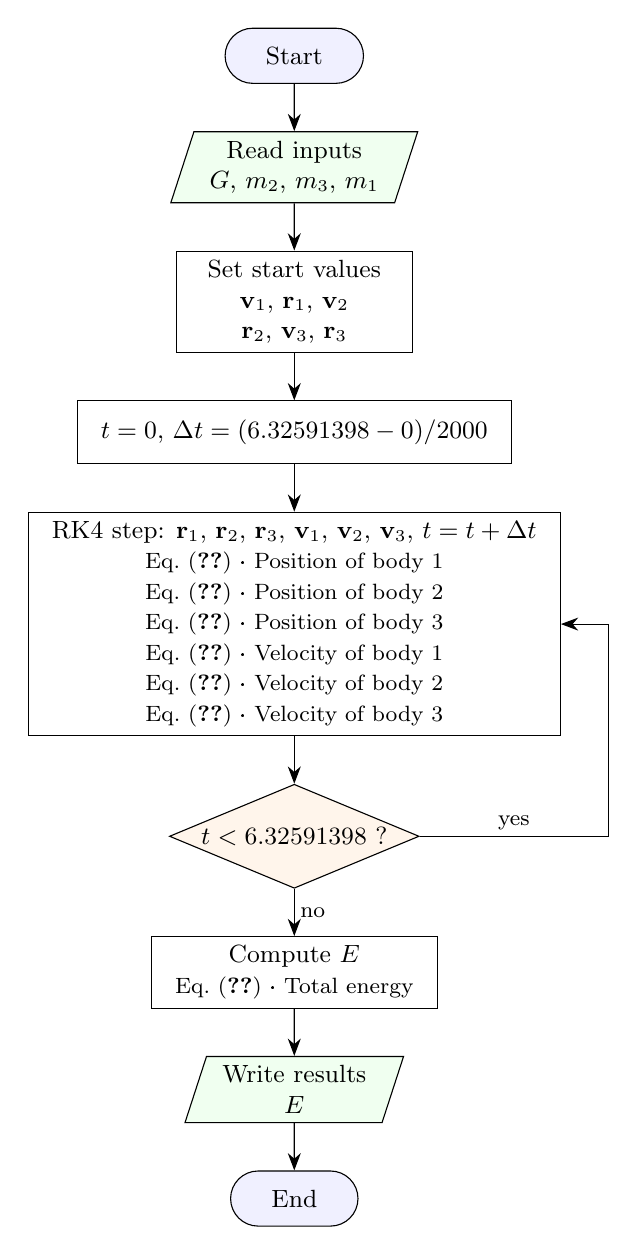
\begin{tikzpicture}[
  node distance=6mm, >={Stealth[length=2.2mm]}, font=\small,
  every node/.style={align=center},
  term/.style={draw, rounded rectangle, minimum height=7mm, inner xsep=5mm, fill=blue!6},
  io/.style={draw, trapezium, trapezium left angle=72, trapezium right angle=108, trapezium stretches body, minimum height=8mm, inner xsep=2mm, fill=green!6},
  proc/.style={draw, rectangle, minimum height=8mm, minimum width=30mm, inner xsep=3mm},
  dec/.style={draw, diamond, aspect=2.4, inner sep=1pt, fill=orange!8},
  lbl/.style={font=\footnotesize, inner sep=2pt}]
  \node[term] (n1) {Start};
  \node[io, below=of n1] (n2) {Read inputs \\ $G$, $m_2$, $m_3$, $m_1$};
  \node[proc, below=of n2] (n3) {Set start values \\ $\mathbf{v}_1$, $\mathbf{r}_1$, $\mathbf{v}_2$ \\ $\mathbf{r}_2$, $\mathbf{v}_3$, $\mathbf{r}_3$};
  \node[proc, below=of n3] (n4) {$t = 0$, $\Delta t = (6.32591398 - 0) / 2000$};
  \node[proc, below=of n4] (n5) {RK4 step: $\mathbf{r}_1$, $\mathbf{r}_2$, $\mathbf{r}_3$, $\mathbf{v}_1$, $\mathbf{v}_2$, $\mathbf{v}_3$, $t = t + \Delta t$ \\ {\footnotesize Eq.~\eqref{eq:position-of-body-1} \textperiodcentered{} Position of body 1} \\ {\footnotesize Eq.~\eqref{eq:position-of-body-2} \textperiodcentered{} Position of body 2} \\ {\footnotesize Eq.~\eqref{eq:position-of-body-3} \textperiodcentered{} Position of body 3} \\ {\footnotesize Eq.~\eqref{eq:velocity-of-body-1} \textperiodcentered{} Velocity of body 1} \\ {\footnotesize Eq.~\eqref{eq:velocity-of-body-2} \textperiodcentered{} Velocity of body 2} \\ {\footnotesize Eq.~\eqref{eq:velocity-of-body-3} \textperiodcentered{} Velocity of body 3}};
  \node[dec, below=of n5] (n6) {$t < 6.32591398$ ?};
  \node[proc, below=of n6] (n7) {Compute $E$ \\ {\footnotesize Eq.~\eqref{eq:total-energy} \textperiodcentered{} Total energy}};
  \node[io, below=of n7] (n8) {Write results \\ $E$};
  \node[term, below=of n8] (n9) {End};
  \coordinate (E) at (current bounding box.east);
  \coordinate (L0) at ([xshift=6mm]E);
  \draw[->] (n1) -- (n2);
  \draw[->] (n2) -- (n3);
  \draw[->] (n3) -- (n4);
  \draw[->] (n4) -- (n5);
  \draw[->] (n5) -- (n6);
  \draw[->] (n6) -- node[lbl, right] {no} (n7);
  \draw[->] (n7) -- (n8);
  \draw[->] (n8) -- (n9);
  \draw[->] (n6.east) -- node[lbl, above] {yes} (n6.east -| L0) |- (n5.east);
\end{tikzpicture}
  \end{adjustbox}
  \caption{Flowchart of the solution procedure}\label{fig:flowchart}
\end{figure}

\bibliographystyle{plain}
\bibliography{references}

\end{document}